% Ternary NCM — draft v0.1 (2026-11-17)
% Every number in this file comes from results_official/*.json; the source file is noted in a comment
% next to each table/figure. Compile with pdflatex + bibtex (e.g. on Overleaf).
\documentclass[11pt]{article}
\usepackage[margin=1in]{geometry}
\usepackage[utf8]{inputenc}
\usepackage[T1]{fontenc}
\usepackage{lmodern}
\usepackage{amsmath,amssymb}
\usepackage{booktabs}
\usepackage{multirow}
\usepackage{graphicx}
\usepackage{xcolor}
\usepackage{pgfplots}
\pgfplotsset{compat=1.17}
\usepackage[numbers,sort&compress]{natbib}
\usepackage[colorlinks=true,linkcolor=blue!50!black,citecolor=blue!50!black,urlcolor=blue!50!black]{hyperref}
\usepackage{caption}
\captionsetup{font=small}

\newcommand{\todo}[1]{\textcolor{red}{[TODO: #1]}}

\title{Can Coarse-to-Fine Text Generators Run on Ternary Weights?\\
\large Post-Training Ternarization of Next-Concept Models Collapses; Quantization-Aware Fine-Tuning Recovers 83\%}
\author{Furkan G\"uven\\F\i rat University, Elaz\u{\i}\u{g}, T\"urkiye\\\texttt{240600205@firat.edu.tr}}
\date{Draft, November 2026}

\begin{document}
\maketitle

\begin{abstract}
Next-Concept Modeling (NCM) generates text coarse-to-fine: a multiscale residual VQ tokenizer turns a sequence
into a hierarchy of discrete codes and a transformer predicts one level per forward pass. We ask whether such a
model survives BitNet~b1.58-style ternary weights ($\{-1,0,+1\}$) with 8-bit activations. Using the official NCM
code and Sudoku-hard checkpoint (86.15\% boards solved on our hardware), we find:
(i)~post-training ternarization collapses the model to \textbf{0\%} for every variant we tried, while INT8 is
lossless and INT4 loses 4.4 points;
(ii)~the collapse is explained by the \emph{magnitude} of the weight perturbation, not by its ternary structure:
isotropic Gaussian noise of the same relative Frobenius error has the same effect, the model tolerates about
0.28 relative error at 50\% solve rate, and even the best per-layer ternary quantizer of Gaussian weights
incurs $\approx$0.44, so no per-layer ternary PTQ can succeed here;
(iii)~quantization-aware fine-tuning from the FP checkpoint, using $\approx$2.5\% of the pretraining sample budget,
recovers \textbf{71.15\,$\pm$\,0.40\%} (3 seeds), i.e.\ 82.6\% of FP;
(iv)~five interventions---distillation from the FP teacher, coarse-level loss reweighting, per-channel scales,
16-bit activations, and keeping the most sensitive block in FP---do not move this ceiling, and a per-puzzle
decomposition shows the remaining gap is spread across levels rather than concentrated in the coarsest
decision. INT8 activations are free. We release code, logs and all numbers. \url{https://github.com/drFurkanGuven/ternary-ncm}
\end{abstract}

% ---------------------------------------------------------------------------------------------------------
\section{Introduction}

Ternary-weight language models such as BitNet~b1.58~\citep{ma2024era} match full-precision (FP) quality at
scale when trained from scratch with quantization in the loop, while cutting weight memory by roughly
$10\times$ and replacing most multiplications with additions. In parallel, non-autoregressive generators have
become competitive for text. Next-Concept Modeling (NCM)~\citep{kumbong2026ncm} is a recent example: it
represents a sequence as 12 levels of residual VQ codes and generates each level in a single parallel forward
pass, reporting 10--31$\times$ faster generation than strong diffusion language models.

The two ideas address different costs---ternary weights reduce the cost of each forward pass, coarse-to-fine
generation reduces the number of passes---so combining them is attractive. It is also not obvious that it
works. In coarse-to-fine models, an error at a coarse level conditions every finer level, and post-training
quantization (PTQ) of related visual coarse-to-fine models already degrades below 4~bits~\citep{litevar,ptq4arvg}.
To our knowledge, no prior work trains or quantizes a coarse-to-fine \emph{text} generator to ternary weights.

We study this question on the one NCM task whose full training data we could reproduce exactly: Sudoku-hard.
Sudoku has an unambiguous success metric (a board is either valid and matches the solution, or not), the
official checkpoint is public, and a solved board requires all 81 cells to be right, which makes the task very
sensitive to small errors.

\paragraph{Contributions.}
\begin{enumerate}
\item A PTQ sweep on the official checkpoint: INT8 is lossless, INT4 costs 4.4 points, and every ternary variant
(absmean per-tensor and per-channel, TWN threshold~\citep{li2016twn}, with and without INT8 activations, on any
subset of layers that includes the input projection or block~0) gives 0\% (\S\ref{sec:ptq}).
\item A mechanism for the collapse. Matched-error Gaussian noise reproduces the quantization curve; the
tolerance threshold ($\approx$0.28--0.35 relative error) lies below the floor of any per-layer
ternary quantizer on Gaussian weights ($\approx$0.44). Damage is not a level-wise cascade: with ground-truth previous levels, the
ternary model is already wrong at nearly every level. Sensitivity is concentrated in the input projection
and the first transformer block (\S\ref{sec:mechanism}).
\item Ternary quantization-aware fine-tuning (QAT) from the FP checkpoint recovers 71.15\,$\pm$\,0.40\% in
55~minutes on one A100 (\S\ref{sec:qat}).
\item Negative results that bound the fine-tuning approach: five interventions leave the ceiling unchanged, and
the gap is a distributed capacity loss, not a coarse-level bottleneck (\S\ref{sec:gap}).
\item Preliminary from-scratch comparisons at small budgets, with an honest account of why our own training recipe
does not reach the paper's FP number (\S\ref{sec:scratch}).
\end{enumerate}

% ---------------------------------------------------------------------------------------------------------
\section{Background}

\paragraph{Next-Concept Modeling.}
NCM~\citep{kumbong2026ncm} has two stages. A multiscale residual VQ-VAE encodes the target sequence into
$K=12$ levels of codes with lengths $l_k \in \{1,2,4,6,9,13,18,26,37,50,67,89\}$ (322 codes in total for
Sudoku); level $k$ quantizes what levels $<k$ left unexplained. A transformer then predicts the codes level by
level, conditioned on a prefix (here the 81-cell puzzle, prefix length 91) and on all coarser levels; positions
within a level are predicted in parallel, so generation takes $K$ forward passes. The VQ decoder maps the final
residual sum back to tokens. Training uses teacher forcing with stochastic corruption of the conditioning
levels and a per-level loss weight $w_k \propto l_k^{-\alpha}$.

\paragraph{BitNet b1.58.}
Each linear layer keeps latent FP weights $W$ and uses, in the forward pass,
\begin{equation}
\widehat W = \gamma\cdot\mathrm{clip}\big(\mathrm{round}(W/\gamma),-1,1\big),\qquad \gamma=\mathrm{mean}|W|,
\end{equation}
with the straight-through estimator (STE)~\citep{bengio2013ste} in the backward pass. Activations are quantized
per token to 8 bits with absmax scaling (W1.58A8)~\citep{ma2024era,wang2023bitnet}.

% ---------------------------------------------------------------------------------------------------------
\section{Experimental setup}
\label{sec:setup}

\paragraph{Model and checkpoint.}
We use the official NCM repository (commit \texttt{c7027427}) and its Sudoku-hard checkpoint without changes to
the architecture. The generator has 25.46M parameters: 8 transformer blocks of width 512, an input projection
(\texttt{wte}) and 12 per-level output heads (\texttt{lm\_heads}). We call the $8\times4=32$ linear layers inside
the blocks (\texttt{attn.c\_attn}, \texttt{attn.c\_proj}, \texttt{mlp.c\_fc}, \texttt{mlp.c\_proj}) the
\emph{body} (25.17M parameters, 99.1\% of all linear-layer weights) and the 13 remaining linears the \emph{io} layers. The VQ-VAE (14.9M)
is frozen and kept in FP throughout.

\paragraph{Data.}
The NCM paper does not ship a training script. We regenerated the Sudoku-hard data with the Sudoku generator
of S-FLM~\citep{deschenaux2026sflm}, which NCM follows for Sudoku (commit \texttt{30def799}, seed 42, 48k train + 2k validation). The 2,000 NCM test puzzles
are identical, in order, to this validation split, with zero overlap with the training split. We hold out
1,000 training puzzles for monitoring.

\paragraph{Evaluation.}
Greedy generation (temperature 0), decoded by the VQ decoder; a puzzle counts as solved if the board is valid and
equals the reference solution. We report the percentage of the 2,000 test puzzles solved. The official checkpoint
gives 86.30\% with the official evaluator on a T4 (paper: 86.1\%) and 86.15\% on an A100 (3 puzzles differ, from
GPU-dependent numerics); we compare every result to the FP number from the same GPU type.

\paragraph{Statistics.}
The binomial standard error of a solve rate near 70\% on 2,000 puzzles is $\approx$1.0 point. For the main QAT
recipe we ran 3 seeds (seed changes data order and corruption noise; the starting weights are identical); the
seed standard deviation is 0.40 points. All other variants are single runs and we only call a difference real
if it clearly exceeds both.

\paragraph{Compute.}
Single Google Colab GPUs (T4 for the PTQ sweep, A100 for training). One 5,000-step QAT run takes 55 minutes on an
A100. One run (block~0 kept FP) took 219 minutes, most likely on a slower GPU type that was not logged; this
affects only wall-clock time.

% ---------------------------------------------------------------------------------------------------------
\section{Post-training ternarization collapses}
\label{sec:ptq}

% Source: results_official/asama1_ptq_sudoku_hard.json (T4, full test)
\begin{table}[t]
\centering
\caption{PTQ of the official Sudoku-hard checkpoint (2,000 test puzzles, T4). Rel.\ err.\ is the
relative Frobenius weight error $\|\widehat W-W\|/\|W\|$ over the quantized layers. Cell accuracy of a
program that copies the 30 clues and fills the rest at random would be $\approx$44\%.}
\label{tab:ptq}
\small
\begin{tabular}{llcrr}
\toprule
Weights & Layers & Rel.\ err. & Solved \% & Cell \% \\
\midrule
FP                         & --   & 0     & 86.30 & 98.35 \\
FP + INT8 act.             & all  & 0     & 86.25 & 98.40 \\
INT8, per-channel          & all  & 0.010 & 86.10 & 98.33 \\
INT4, per-channel          & all  & 0.189 & 81.90 & 97.83 \\
INT4, per-channel          & body & 0.190 & 83.00 & 97.94 \\
\midrule
Ternary absmean, per-tensor & all  & 0.559 & 0.00 & 22.61 \\
Ternary absmean, per-tensor & body & 0.559 & 0.00 & 27.49 \\
\quad + INT8 act.           & body & 0.559 & 0.00 & 27.37 \\
Ternary absmean, per-channel & body & 0.540 & 0.00 & 23.44 \\
Ternary TWN, per-channel    & body & 0.465 & 0.00 & 18.37 \\
Ternary absmean, per-tensor & attention only & 0.540 & 0.00 & 41.10 \\
Ternary absmean, per-tensor & MLP only       & 0.568 & 0.00 & 40.00 \\
Ternary absmean, per-tensor & io only (13 layers, 0.9\%) & -- & 0.00 & -- \\
\bottomrule
\end{tabular}
\end{table}

Table~\ref{tab:ptq} shows the PTQ sweep. Eight-bit weights are lossless and 4-bit weights cost 4.4 points,
consistent with PTQ results on other generators. Every ternary variant solves no puzzle at all, and cell
accuracy (18--41\%) is below what copying the clues and guessing would give. Restricting ternarization to
attention, to the MLPs, or to the 13 io layers does not help.

\subsection{Mechanism}
\label{sec:mechanism}

We ran a measurement-only diagnostic on the first 500 (curve) or 256 (sweeps) test puzzles on an A100
(FP: 85.0\% on the first 500).

% Source: results_official/asama2b_diag_ptq_mechanism.json, A_error_curve_first500
\begin{figure}[t]
\centering
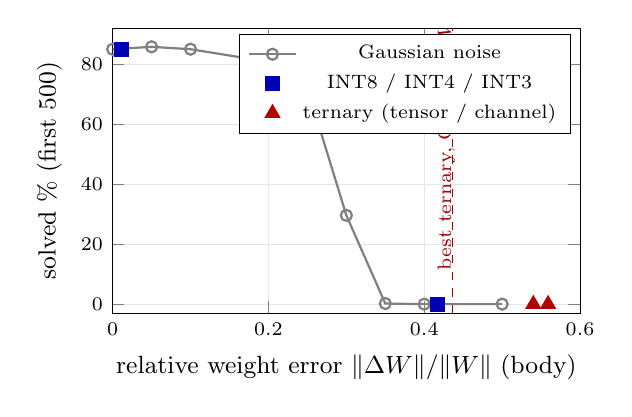
\begin{tikzpicture}
\begin{axis}[
  width=0.62\linewidth, height=5.2cm,
  xlabel={relative weight error $\|\Delta W\|/\|W\|$ (body)},
  ylabel={solved \% (first 500)},
  xmin=0, xmax=0.6, ymin=-3, ymax=92,
  legend style={font=\scriptsize, at={(0.98,0.98)}, anchor=north east},
  grid=major, grid style={gray!20},
  tick label style={font=\scriptsize}, label style={font=\small}]
\addplot[thick, mark=o, color=gray] coordinates {
  (0,85.0) (0.05,85.8) (0.1,85.0) (0.2,80.8) (0.25,72.0) (0.3,29.6) (0.35,0.2) (0.4,0.0) (0.5,0.0)};
\addlegendentry{Gaussian noise}
\addplot[only marks, mark=square*, mark size=2.5pt, color=blue!70!black] coordinates {
  (0.011,84.8) (0.19,83.4) (0.417,0.0)};
\addlegendentry{INT8 / INT4 / INT3}
\addplot[only marks, mark=triangle*, mark size=3pt, color=red!70!black] coordinates {
  (0.559,0.0) (0.54,0.0)};
\addlegendentry{ternary (tensor / channel)}
\draw[dashed, red!60!black] (axis cs:0.436,-3) -- (axis cs:0.436,92);
\node[font=\scriptsize, red!60!black, anchor=south west, rotate=90] at (axis cs:0.452,8) {best ternary, Gaussian $W$};
\end{axis}
\end{tikzpicture}
\caption{Solve rate as a function of relative weight error on the 32 body layers. Gaussian noise with matched
per-layer error (grey) predicts integer quantization (blue) and ternary (red). The dashed line is the
lowest relative error any per-layer ternary quantizer can reach on Gaussian weights (0.436, computed numerically
with optimal threshold and scale); it lies beyond the point where the model fails.}
\label{fig:errcurve}
\end{figure}

\paragraph{Error magnitude, not ternary structure.}
Figure~\ref{fig:errcurve} plots solve rate against the relative Frobenius error of the body weights. Adding
isotropic Gaussian noise of a prescribed relative error to each layer reproduces the quantization results:
INT4 (0.19) gives 83.4\% and noise at 0.20 gives 80.8\%; INT3 (0.42) and noise at 0.40 both give 0\%. The model
reaches 50\% solved at a relative error of about 0.28 and is essentially at 0\% from 0.35. For Gaussian weights,
absmean ternarization has relative error 0.513 and the best possible per-layer ternary quantizer (threshold
search, $L_2$-optimal scale) 0.436; on the real checkpoint we measure 0.46--0.56 (Table~\ref{tab:ptq}). Ternary PTQ therefore cannot
succeed on this model without reducing error below the tolerance by roughly a factor of 1.5, which no per-layer
rounding scheme can do. This framing also explains why calibration-free refinements (per-channel scales, TWN
thresholds) did not help: they move the error by a few hundredths.

% Source: per_level in asama2b_diag_ptq_mechanism.json
\paragraph{No level-wise cascade.}
A natural hypothesis for a coarse-to-fine model is error accumulation across levels: a slightly wrong coarse
code derails the finer ones. The data do not support it. With teacher forcing (ground-truth codes for all
previous levels) the ternary model's per-level accuracy is already 0.08--0.18 on levels 0--10 apart from the
trivial ones (level 0: 0.116) and 0.43 on the finest level, close to its accuracy in free generation; 446 of 500 puzzles diverge from the FP
model's codes at level~0. (Levels 1 and 4 are nearly deterministic given the prefix and stay at 0.91 and 1.0
for all models.) The damage happens inside each forward pass.

\paragraph{Damage accumulates with depth, sensitivity sits at the input.}
The relative drift of the hidden state from FP grows from 0.37 after block~0 to 1.01 after block~7.
Ternarizing single layers or blocks (first 256 puzzles; ternarizing a single output head gives 84.4--85.6\%,
i.e.\ FP level) isolates the sensitive parts: the input projection
\texttt{wte} alone, or either attention layer of block~0 alone, gives 0\%; block~0 alone gives 0\%, block~1
24.6\%, and blocks 2--7 individually 70--77\%. The earlier ``io layers only $\to$ 0\%'' result is due to
\texttt{wte}; each output head alone is harmless ($\approx$85\%). Ternarizing the last $k$ blocks degrades
gracefully (73.4, 57.4, 34.0, 3.1\% for $k=1..4$), while any set containing block~0 gives 0\%.

\paragraph{Codes are not unique.}
INT8 weights solve 84.8\% but reproduce the FP model's exact code sequence for only 41.8\% of puzzles (noise at
0.05: 85.8\% solved, 1.6\% identical codes). Many code paths decode to the same correct board, so code-level
agreement with FP is not a useful target for distillation or calibration.

% ---------------------------------------------------------------------------------------------------------
\section{Ternary quantization-aware fine-tuning}
\label{sec:qat}

\paragraph{Recipe (E3).}
Starting from the FP checkpoint, we replace the 32 body linears by W1.58A8 layers (absmean per-tensor ternary
weights, per-token INT8 absmax activations, STE), keep the io layers in FP, and fine-tune with the NCM
teacher-forcing loss. Since no training script is released, we had to choose the hyperparameters the paper does
not state for Sudoku: linearly decreasing conditioning corruption with mean 0.5 (0.75 at the coarsest
conditioning level to 0.25 at the finest), $\alpha=0$, batch 256, AdamW with peak learning rate $10^{-4}$, 100
warm-up steps and cosine decay to $10^{-5}$. We verified that our teacher-forcing input builder reproduces the
official greedy generator's predictions exactly (100\% agreement at every level), and the official FP model has
teacher-forcing loss 0.105 on our data.

% Source: asama2b_E3_ternary_ft.json, _5k.json, _seeds.json, _kd_partial.json, _alpha1.json, _a16.json, _pc.json, _b0fp.json
\begin{table}[t]
\centering
\caption{Ternary QAT fine-tuning from the FP checkpoint (A100, full test). 5,000 steps $\times$ 256 sequences is
$\approx$2.5\% of the NCM pretraining sample budget (50k steps $\times$ 1024). Seed std of the main recipe is
0.40; binomial SE $\approx$1.0.}
\label{tab:qat}
\small
\begin{tabular}{lrrl}
\toprule
Run & Steps & Solved \% & Note \\
\midrule
Official FP (A100)          & --    & 86.15 & reference \\
Ternary PTQ (body)          & 0     & 0.00  & Table~\ref{tab:ptq} \\
\midrule
E3                          & 1,500 & 69.70 & 15 min \\
\textbf{E3-long} (3 seeds)  & 5,000 & \textbf{71.15\,$\pm$\,0.40} & 71.60 / 70.85 / 71.00; 82.6\% of FP \\
\midrule
\quad + distillation from FP teacher, $\lambda$ warm-up & 2,000 & -- & stopped; equal to E3-long at 1k/2k steps \\
\quad $\alpha=1$ (coarsest level weighted 27$\times$ more) & 5,000 & 69.05 & worse ($\approx$5 seed std) \\
\quad W1.58A16 (no activation quantization)               & 5,000 & 71.05 & INT8 activations are free \\
\quad per-channel ternary scale                         & 5,000 & 71.80 & within noise \\
\quad block 0 kept FP (28 ternary body layers)          & 5,000 & 71.30 & within noise \\
\bottomrule
\end{tabular}
\end{table}

% Source: during_training_test_subset_256 and holdout_tf_loss in asama2b_E3_ternary_ft_5k.json and _seeds.json
\begin{figure}[t]
\centering
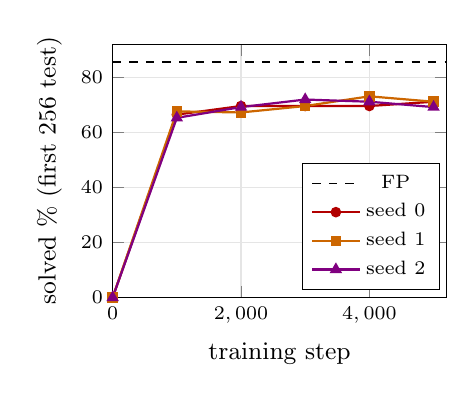
\begin{tikzpicture}
\begin{axis}[
  width=0.48\linewidth, height=4.8cm,
  xlabel={training step}, ylabel={solved \% (first 256 test)},
  xmin=0, xmax=5200, ymin=0, ymax=92, grid=major, grid style={gray!20},
  legend style={font=\scriptsize, at={(0.98,0.03)}, anchor=south east},
  tick label style={font=\scriptsize}, label style={font=\small},
  scaled x ticks=false, xticklabel style={/pgf/number format/1000 sep={,}}]
\addplot[dashed, black] coordinates {(0,85.5) (5200,85.5)};
\addlegendentry{FP}
\addplot[thick, mark=*, mark size=1.5pt, color=red!70!black] coordinates {
  (0,0) (1000,66.41) (2000,69.53) (3000,69.53) (4000,69.53) (5000,71.09)};
\addlegendentry{seed 0}
\addplot[thick, mark=square*, mark size=1.5pt, color=orange!80!black] coordinates {
  (0,0) (1000,67.58) (2000,67.19) (3000,69.53) (4000,73.05) (5000,71.09)};
\addlegendentry{seed 1}
\addplot[thick, mark=triangle*, mark size=1.8pt, color=violet] coordinates {
  (0,0) (1000,65.23) (2000,69.14) (3000,71.88) (4000,71.09) (5000,69.14)};
\addlegendentry{seed 2}
\end{axis}
\end{tikzpicture}\hfill
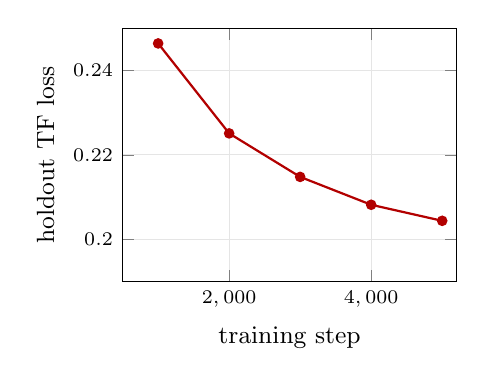
\begin{tikzpicture}
\begin{axis}[
  width=0.48\linewidth, height=4.8cm,
  xlabel={training step}, ylabel={holdout TF loss},
  xmin=500, xmax=5200, ymin=0.19, ymax=0.25, grid=major, grid style={gray!20},
  tick label style={font=\scriptsize}, label style={font=\small},
  scaled x ticks=false, xticklabel style={/pgf/number format/1000 sep={,}},
  yticklabel style={/pgf/number format/fixed, /pgf/number format/precision=2}]
\addplot[thick, mark=*, mark size=1.5pt, color=red!70!black] coordinates {
  (1000,0.2464) (2000,0.2251) (3000,0.2148) (4000,0.2082) (5000,0.2044)};
\end{axis}
\end{tikzpicture}
\caption{E3-long. Left: solve rate on the first 256 test puzzles during training, three seeds; it plateaus after
$\approx$2,000 steps. Right: teacher-forcing loss on held-out training puzzles (seed 0) keeps decreasing. The
initial point (step 0, 0\%) is the ternary PTQ model.}
\label{fig:curves}
\end{figure}

Table~\ref{tab:qat} and Figure~\ref{fig:curves} summarize the results. Fine-tuning lifts the ternary model from
0\% to 49.6\% (first 256 puzzles) within 250 steps and to 69.7\% (full test) within 1,500 steps. Tripling the
budget adds only 1.5--2 points: the solve rate plateaus after about 2,000 steps although the held-out
teacher-forcing loss continues to fall. Three seeds give 71.60, 70.85 and 71.00\%, i.e.\ 71.15\,$\pm$\,0.40\%,
82.6\% of the FP model. Fine-tuning shifts the weights well past the PTQ tolerance (Section~\ref{sec:mechanism}):
QAT does not make ternary rounding more accurate, it moves the network to a different solution that works under
ternary constraints, in line with observations that sub-3-bit fine-tuning substantially changes the weight
distribution~\citep{liu2025paretoq}.

% ---------------------------------------------------------------------------------------------------------
\section{Where is the remaining gap?}
\label{sec:gap}

\paragraph{Interventions that did not help.}
Each of the following targets one hypothesis for the 15-point gap; none moves the result beyond the seed
spread (Table~\ref{tab:qat}).
\emph{Distillation} from the FP teacher with gradual quantization ($\lambda$ ramped over 500 steps) matched E3-long
at steps 1,000 and 2,000 (66.8 / 68.8 vs.\ 66.4 / 69.5\% on 256 puzzles) and was stopped; the ramp only delays the
loss spike to the point where $\lambda=1$.
\emph{Coarse-level reweighting} ($\alpha=1$, which weights the single coarsest code 27$\times$ more than with
$\alpha=0$) left coarsest-level accuracy at $\approx$80\% and hurt finer levels (69.05\%).
\emph{16-bit activations} (W1.58A16) gave 71.05\%: the gap comes from ternary weights, and INT8 activations cost
nothing on this model.
\emph{Per-channel scales} ($\widehat W=\mathrm{diag}(\gamma)\,T$) lowered held-out loss slightly (0.195 vs.\ 0.204)
without changing the solve rate (71.80\%).
\emph{Keeping block~0 in FP}, the most PTQ-sensitive block, gave 71.30\% with identical held-out loss (0.204).

% Source: asama2b_diag_coarse_code_decomposition.json
\paragraph{The gap is not in the coarsest code.}
On the full test set we compared the generated coarsest code (one code, level 0) with the code the tokenizer
assigns to the true solution. The FP model gets it right for 85.5\% of puzzles and E3-long for 76.7\%.
Conditional solve rates are $P(\text{solved}\mid\text{correct})=88.1\%$ vs.\ 74.6\% and
$P(\text{solved}\mid\text{wrong})=74.8\%$ vs.\ 61.8\%. A wrong coarsest code still leads to the correct board most
of the time, consistent with the non-uniqueness of codes above. If the ternary model had the FP model's
coarsest-code accuracy, it would solve $0.855\cdot74.6+0.145\cdot61.8\approx72.7\%$, only 1.1 points more: the
coarsest decision explains about 1 of the 14.5 points. The rest is a lower conditional success at every
subsequent level, i.e.\ a distributed loss of capacity. This also explains why reweighting the coarsest level
and distilling level-wise targets did not help.

Together with the block-0 result, this suggests that within a 2.5\% fine-tuning budget the 25M-parameter body
simply has less usable capacity when ternary. Whether a longer budget, ternary pretraining from scratch at the
paper's budget, or a larger body closes the gap is open; BitNet results suggest the gap shrinks with
scale~\citep{ma2024era}, while fine-tuning studies on LLMs report that it can widen with
scale~\citep{bitdistill}.

% ---------------------------------------------------------------------------------------------------------
\section{Training from scratch at small budgets}
\label{sec:scratch}

% Source: asama2b_E1_fp_scratch*.json, asama2b_E2_ternary_scratch*.json, asama2b_diag_E1_long_train_vs_test.json
\begin{table}[t]
\centering
\caption{Training from scratch with our recipe (A100, full test, single seed). Budgets are 2\% and 6\% of the
paper's sample budget. Holdout loss is teacher-forcing loss on clean inputs.}
\label{tab:scratch}
\small
\begin{tabular}{lrrrl}
\toprule
Run & Steps & Solved \% & Holdout loss & Note \\
\midrule
FP (E1)        & 4,000  & 21.75 & 0.378 & \\
Ternary (E2)   & 4,000  & 16.45 & 0.411 & 76\% of FP \\
FP (E1-long)   & 12,000 & 25.65 & 0.436 & loss minimum 0.374 at 6k, then rises \\
Ternary (E2-long) & 12,000 & 22.75 & 0.369 & 89\% of FP; loss flat from 8k \\
\bottomrule
\end{tabular}
\end{table}

Table~\ref{tab:scratch} reports from-scratch training with the same recipe (peak learning rate
$3\cdot10^{-4}$, 500 warm-up steps). Both models remain far below the paper's 86.1\%, and we want to be explicit
that this is a limitation of our recipe rather than of NCM: at 12k steps the FP model solves 98.6\% of the first
500 \emph{training} puzzles but only 24.8\% of the first 500 test puzzles, i.e.\ it memorizes. We guessed several
settings (batch 256 vs.\ 1024, corruption schedule, $\alpha$, absence of data augmentation), and a random-rate
corruption variant inspired by the official LM1B config did worse (18.35\%) while lowering teacher-forcing loss,
which also shows that teacher-forcing loss is not a reliable proxy for solve rate here.

Within this recipe two observations are robust enough to report. The ternary model needs roughly
1.3--1.6$\times$ more steps to reach the same held-out loss as FP, and the relative gap in solve rate narrows from
76\% to 89\% of FP between 4k and 12k steps. At 12k steps the FP model's held-out loss rises while the ternary
model's stays flat and ends lower (0.369 vs.\ 0.436), i.e.\ the ternary constraint acts as a regularizer against
memorization. These are single-seed results at budgets far below the paper's and should be read as preliminary.

% ---------------------------------------------------------------------------------------------------------
\section{Memory}
\label{sec:memory}

Ternary weights need $\log_2 3\approx1.58$ bits per weight (2 bits with simple packing). The body of the Sudoku
generator shrinks from 50.3\,MB (FP16) to 5.0\,MB at 1.58 bits or 6.3\,MB at 2 bits; the remaining FP parameters (io layers, norms, embeddings) add
$\approx$0.6\,MB. The frozen VQ-VAE (14.9M parameters) is not quantized here; only its decoder is needed at
inference. We do not report speed or energy: our ternary layers are simulated in FP arithmetic, and realizing the
savings requires dedicated kernels.

% ---------------------------------------------------------------------------------------------------------
\section{Related work}

\paragraph{Ternary and low-bit language models.}
BitNet~\citep{wang2023bitnet} and BitNet~b1.58~\citep{ma2024era} train ternary-weight LLMs from scratch with
8-bit activations. ParetoQ~\citep{liu2025paretoq} compares 1--4-bit QAT under a unified framework and reports a
transition between 2 and 3 bits, below which fine-tuned weights move far from their pretrained values.
Fine-tuning FP LLMs into 1.58-bit models leaves a gap that BitNet Distillation~\citep{bitdistill} closes with
architectural refinement, continued pretraining and distillation. Post-training ternarization of LLMs is an
active area~\citep{pt2llm}; our error-tolerance analysis gives a simple test for when such methods can or cannot
work on a given model.

\paragraph{Quantization of non-autoregressive and coarse-to-fine generators.}
For visual autoregressive models with next-scale prediction (VAR~\citep{tian2024var}), quantization work is PTQ
and degrades below 4--6 bits~\citep{litevar,ptq4arvg}. Diffusion language models have been studied with PTQ
down to 4 bits~\citep{lin2025dllmquant}. Ternary QAT has been shown for diffusion transformers in
images~\citep{lu2024terdit}. We are not aware of ternary training or quantization of coarse-to-fine \emph{text}
generators such as NCM~\citep{kumbong2026ncm} (literature search as of November 2026).

% ---------------------------------------------------------------------------------------------------------
\section{Limitations}

\begin{itemize}
\item \textbf{One task, one small model.} All results are on Sudoku-hard with a 25M-parameter generator. Sudoku is
an all-or-nothing metric and may be more sensitive to weight error than open-ended text. The official NCM text
checkpoints (e.g.\ LM1B, OWT) are the obvious next step.
\item \textbf{Unofficial training recipe.} Fine-tuning hyperparameters and all from-scratch settings are our
guesses; from-scratch FP training does not reproduce the paper.
\item \textbf{Seeds.} Only the main QAT recipe has 3 seeds; all variants and from-scratch runs are single runs.
\item \textbf{Simulated quantization.} No speed or energy measurements.
\item \textbf{Diagnostic subsets.} Mechanism experiments use the first 256 or 500 test puzzles.
\end{itemize}

% ---------------------------------------------------------------------------------------------------------
\section{Conclusion}

Ternary weights and coarse-to-fine generation can be combined, but not after the fact. On NCM Sudoku-hard,
ternary PTQ fails for a simple quantitative reason---the model tolerates about 0.3 relative weight error and
ternary rounding cannot go below about 0.44---while a short quantization-aware fine-tuning recovers 83\% of FP
performance with free INT8 activations. The remaining gap is a distributed capacity loss that the obvious
fine-tuning fixes do not touch, which points to ternary pretraining at full budget and to larger models as the
next experiments.

\paragraph{Reproducibility.}
Code (Colab notebooks, quantization and training modules), all logs, and a JSON file for every number in this
paper are available at \url{https://github.com/drFurkanGuven/ternary-ncm}. External code is pinned to commits (NCM \texttt{c7027427}, S-FLM
generator \texttt{30def799}).

\bibliographystyle{plainnat}
\bibliography{refs}

\end{document}
